\section{Struktur des Prozessmodells} \label{Prozessmodellstruktur}
	
	\begin{wrapfigure}{r}{0.45\textwidth}
		\centering
		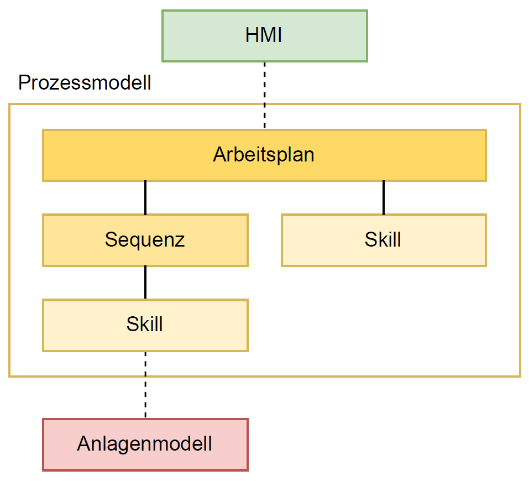
\includegraphics[width=0.4\textwidth]{08_Prozessmodell/Grundstruktur}
		\captionsetup{justification=centering}
		\caption{Grundstruktur des Prozessmodells}
		\label{fig:Prozessmodellgrundstruktur}
	\end{wrapfigure} \par
	Die grundlegende Struktur des Prozessmodells lässt sich klar und einfach definieren: Der gesamte Prozess wird durch einen Arbeitsplan abgebildet. Dieser besteht aus verschiedenen Sequenzen und Skills, wobei Sequenzen aus mehreren Skills zusammengesetzt sind (Abb. \ref{fig:Prozessmodellgrundstruktur}).
	\\
	Skills repräsentieren die grundlegenden Funktionalitäten einzelner Komponenten, während Sequenzen die Funktionen des Gesamtsystems oder von Teilsystemen darstellen.
	\\
	Das Prozessmodell verfügt über zwei zentrale Schnittstellen: zum Anlagenmodell und zum HMI. Die Interaktion mit dem Anlagenmodell erfolgt dabei ausschliesslich über die Skills. Über das HMI wird der Arbeitsplan gesteuert, wodurch eine intuitive Bedienung und Anpassung des Prozesses ermöglicht werden soll.
	\\
	Die Struktur des Prozessmodells beeinflusst massgeblich die Flexibilität der Erstellung und Nutzung eines Arbeitsplans. Es stellt sich die Frage, ob das Ziel darin besteht, über ein HMI flexibel Abläufe zusammenstellen zu können, oder ob lediglich ein vordefinierter Ablauf gestartet werden soll. Beide Ansätze erfordern unterschiedliche Programmstrukturen:
	
	\textbf{Ansatz 1: } Vordefinierte Abläufe (Abb. \ref{fig:Ansatz_1})
	\vspace{2mm}
	\\
	Hier werden feste Abläufe vorab definiert und können mit minimalem Aufwand gestartet werden. Dies erfordert eine weniger dynamische, dafür jedoch robuste Struktur, die auf vorgefertigten Arbeitsplänen basiert.
	
	\newpage
	
	\textbf{Ansatz 2: }Flexible Erstellung über das HMI (Abb. \ref{fig:Ansatz_2})
	\vspace{2mm}
	\\
	Diese Variante ermöglicht eine dynamische Konfiguration von Abläufen direkt über die Benutzeroberfläche. Hierfür ist eine modulare und erweiterbare Programmstruktur notwendig, die es erlaubt, Sequenzen und Skills zur Laufzeit zu definieren und zu kombinieren. Folgende Schemas zeigen grob die Struktur dieser Ansätze: 
	
	\begin{figure}[h!]
		\centering
		\begin{subfigure}[b]{0.42\textwidth}
			\centering
			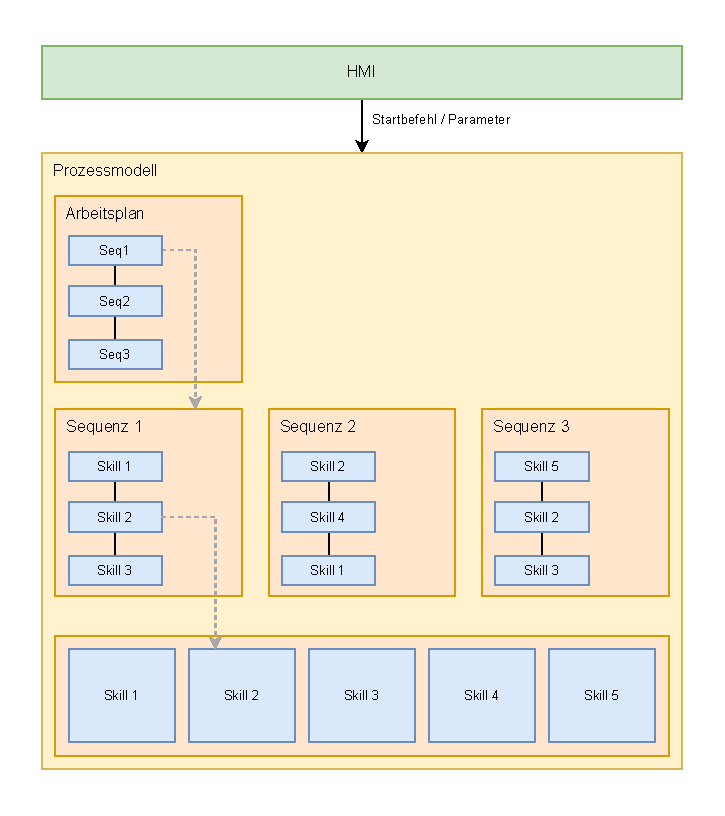
\includegraphics[width=\textwidth]{08_Prozessmodell/Ansatz_1}
			\caption{Ansatz 1}
			\label{fig:Ansatz_1}
		\end{subfigure}
		\hfill
		\begin{subfigure}[b]{0.42\textwidth}
			\centering
			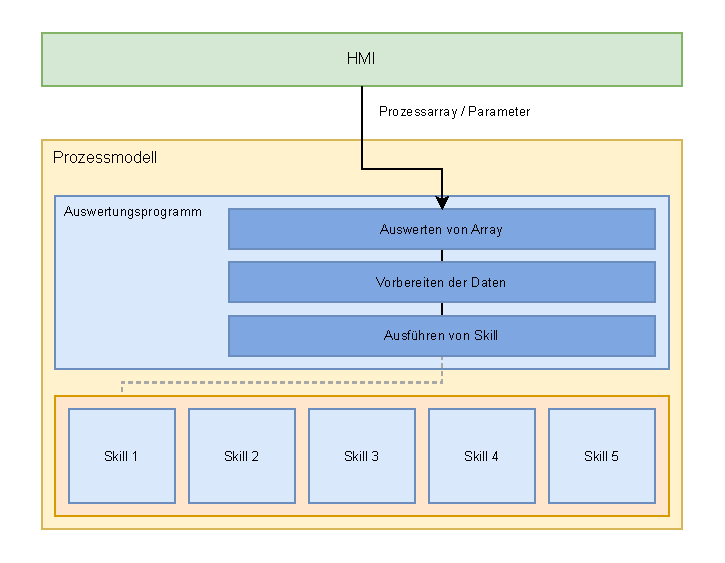
\includegraphics[width=\textwidth]{08_Prozessmodell/Ansatz_2}
			\caption{Ansatz 2}
			\label{fig:Ansatz_2}
		\end{subfigure}
		\caption{Ansatzvergleich}
		\label{fig:Ansatzvergleich}
	\end{figure}
	
	Ansatz 1 folgt einer bewährten Methode, wie sie bereits in TwinCAT für Rezeptursteuerungen eingesetzt wird. Hier werden die Prozessabläufe durch vordefinierte Schrittabfolgen realisiert, die je nach Bedarf ausgelöst werden. Über das HMI erfolgt lediglich der Start des Prozesses sowie die Eingabe der erforderlichen Parameter.
	
	\begin{tabularx}{\textwidth}{@{}>{}p{5em} X@{}}
	Vorteile: 	& 	\vspace{-3mm} \begin{itemize}
						\item Klare und übersichtliche Struktur.
						\item Einfache Implementierung dank zahlreicher Referenzen und standardisierter Konzepte.
						\item Schnelle Umsetzbarkeit.
					\end{itemize}
	\\
	Nachteile: 	& 	\vspace{-3mm} \begin{itemize}
						\item Eingeschränkte Flexibilität: Abläufe können nicht dynamisch angepasst oder neu erstellt werden.
						\item Begrenzte Übertragbarkeit auf vollständig flexible Prozesse.
					\end{itemize}
	\\
	\end{tabularx} 
	
	Ansatz 2 bietet eine wesentlich flexiblere Gestaltung der Prozessabläufe. Über das HMI können Abläufe frei durch die Kombination von Skills und Sequenzen definiert werden. Jeder Skill wird durch eine eindeutige Nummer repräsentiert, während Sequenzen als Arrays von Nummern aufgebaut sind, die den Prozessablauf abbilden. Ein Programm im Prozessmodell analysiert dieses Array und führt die Skills in der definierten Reihenfolge aus.
	
	\begin{tabularx}{\textwidth}{@{}>{}p{5em} X@{}}
		Vorteile: 	& 	\vspace{-3mm} \begin{itemize}
							\item Hohe Flexibilität: Prozesse können individuell und dynamisch über die HMI erstellt werden.
							\item Anpassbar an variable Anforderungen oder neue Arbeitsabläufe.
		\end{itemize}
		\\
		Nachteile: 	& 	\vspace{-3mm} \begin{itemize}
							\item Höhere Komplexität bei der Implementierung.
							\item Mögliche Herausforderungen bei parallelen Prozessen, insbesondere in Bezug auf Synchronisation und Timing.
		\end{itemize}
		\\
	\end{tabularx} 
	
	\newpage
	
	Zunächst wird die Struktur gemäss Ansatz 1 umgesetzt, da sie bewährt und schnell realisierbar ist. Je nach dem welche Erfahrungen mit dieser Struktur gemacht werden, kann in einer zweiten Iteration auf Ansatz 2 umgestellt werden, um mehr Flexibilität zu ermöglichen. Die Skills bleiben in beiden Ansätzen unverändert und können somit nahtlos übernommen werden.
	
	\subsection{Struktur eines Arbeitsplans nach Ansatz 1} \label{Arbeitsplanstruktur}
	
		\begin{wrapfigure}{r}{0.55\textwidth}
			\centering
			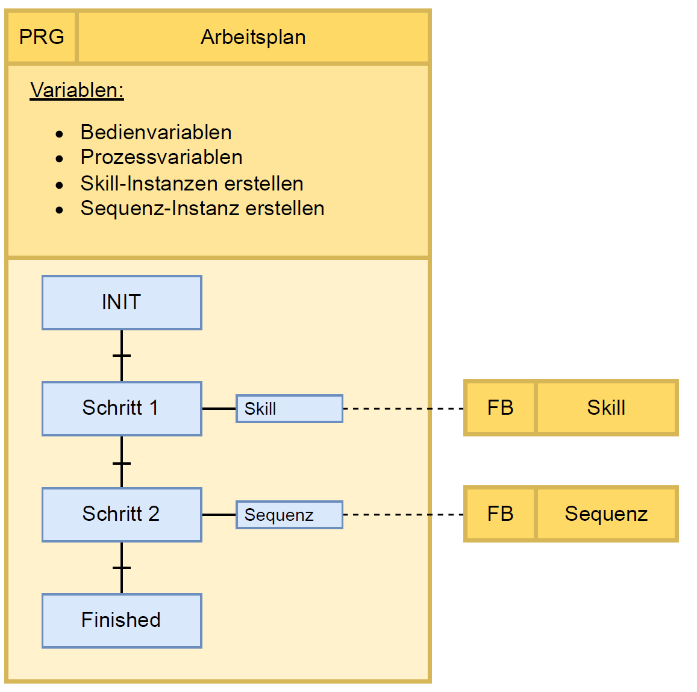
\includegraphics[width=0.5\textwidth]{08_Prozessmodell/Arbeitsplanstruktur}
			\captionsetup{justification=centering}
			\caption{Struktur des Arbeitsplans}
			\label{fig:Arbeitsplanstruktur}
		\end{wrapfigure} \par	
		Die Struktur eines Arbeitsplans ist klar und übersichtlich. Ein Arbeitsplan wird als eigenständiges Programm (PRG) definiert, das den Prozess in Form eines Schrittablaufs abbildet. Jeder Schritt führt entweder Skills oder Sequenzen aus. Innerhalb des Programms werden verschiedene Variablen und Funktionsbausteine instanziiert, um den Ablauf zu steuern.
		\\
		Die Bedienvariablen dienen zum Starten, Stoppen und Zurücksetzen des Schrittablaufs. Prozessvariablen enthalten alle prozessrelevanten Informationen, die für die Ausführung des Arbeitsplans erforderlich sind. Zusätzlich müssen im Arbeitsplan alle benötigten Skills und Sequenzen instanziiert werden. Dabei werden ausschliesslich die Skills instanziiert, die im Schrittablauf des Arbeitsplans tatsächlich verwendet werden. Skills, die innerhalb von Sequenzen genutzt werden, werden direkt in den Sequenzen selbst instanziiert.
		
	\subsection{Struktur von Sequenzen} \label{Sequenzstruktur}
		
		Sequenzen werden analog zu Skills als Funktionsbausteine definiert, wobei auch hier das Ziel darin besteht, eine einheitliche Struktur bereitzustellen. Ein zentraler Bestandteil dieser Struktur ist die Definition der Schnittstellen einer Sequenz, die in zwei Kategorien unterteilt wurden. Die Steuerungselemente sind für die Bedienung der Sequenz vorgesehen. Die Sequenz wird gestartet, gestoppt oder resettet. Zusätzlich werden auch Informationen über den Zustand der Sequenz angegeben.  Der Arbeitsplan startet hierbei die Sequenz oder resettet diese. Über den Zustand weiss der Arbeitsplan, wann eine Sequenz abgeschlossen wurde. 
		\\
		Die Betriebsvariablen sind für den Betrieb der Sequenz angedacht. Im Gegensatz zum Skill wurden die Prozessparameter hier direkt in die Betriebsvariablen integriert.
		\\
		Die Struktur der Sequenz hat während der Entwicklung mehrere Iterationen durchlaufen. In der Dokumentation wird jedoch ausschliesslich der aktuelle Stand beschrieben, da nicht alle Entwicklungsschritte detailliert erläutert werden. Während der Entwicklungs- und Testphase wurden zahlreiche Erkenntnisse und Erfahrungen gesammelt, die die Struktur massgeblich beeinflusst haben. Viele Anpassungen waren notwendig, um TwinCAT-spezifische Probleme zu bewältigen. Dabei konnte wertvolles Know-how über TwinCAT und dessen Arbeitsweise gewonnen werden.
		
		\newpage
		
		\begin{figure}[H]
			\centering
			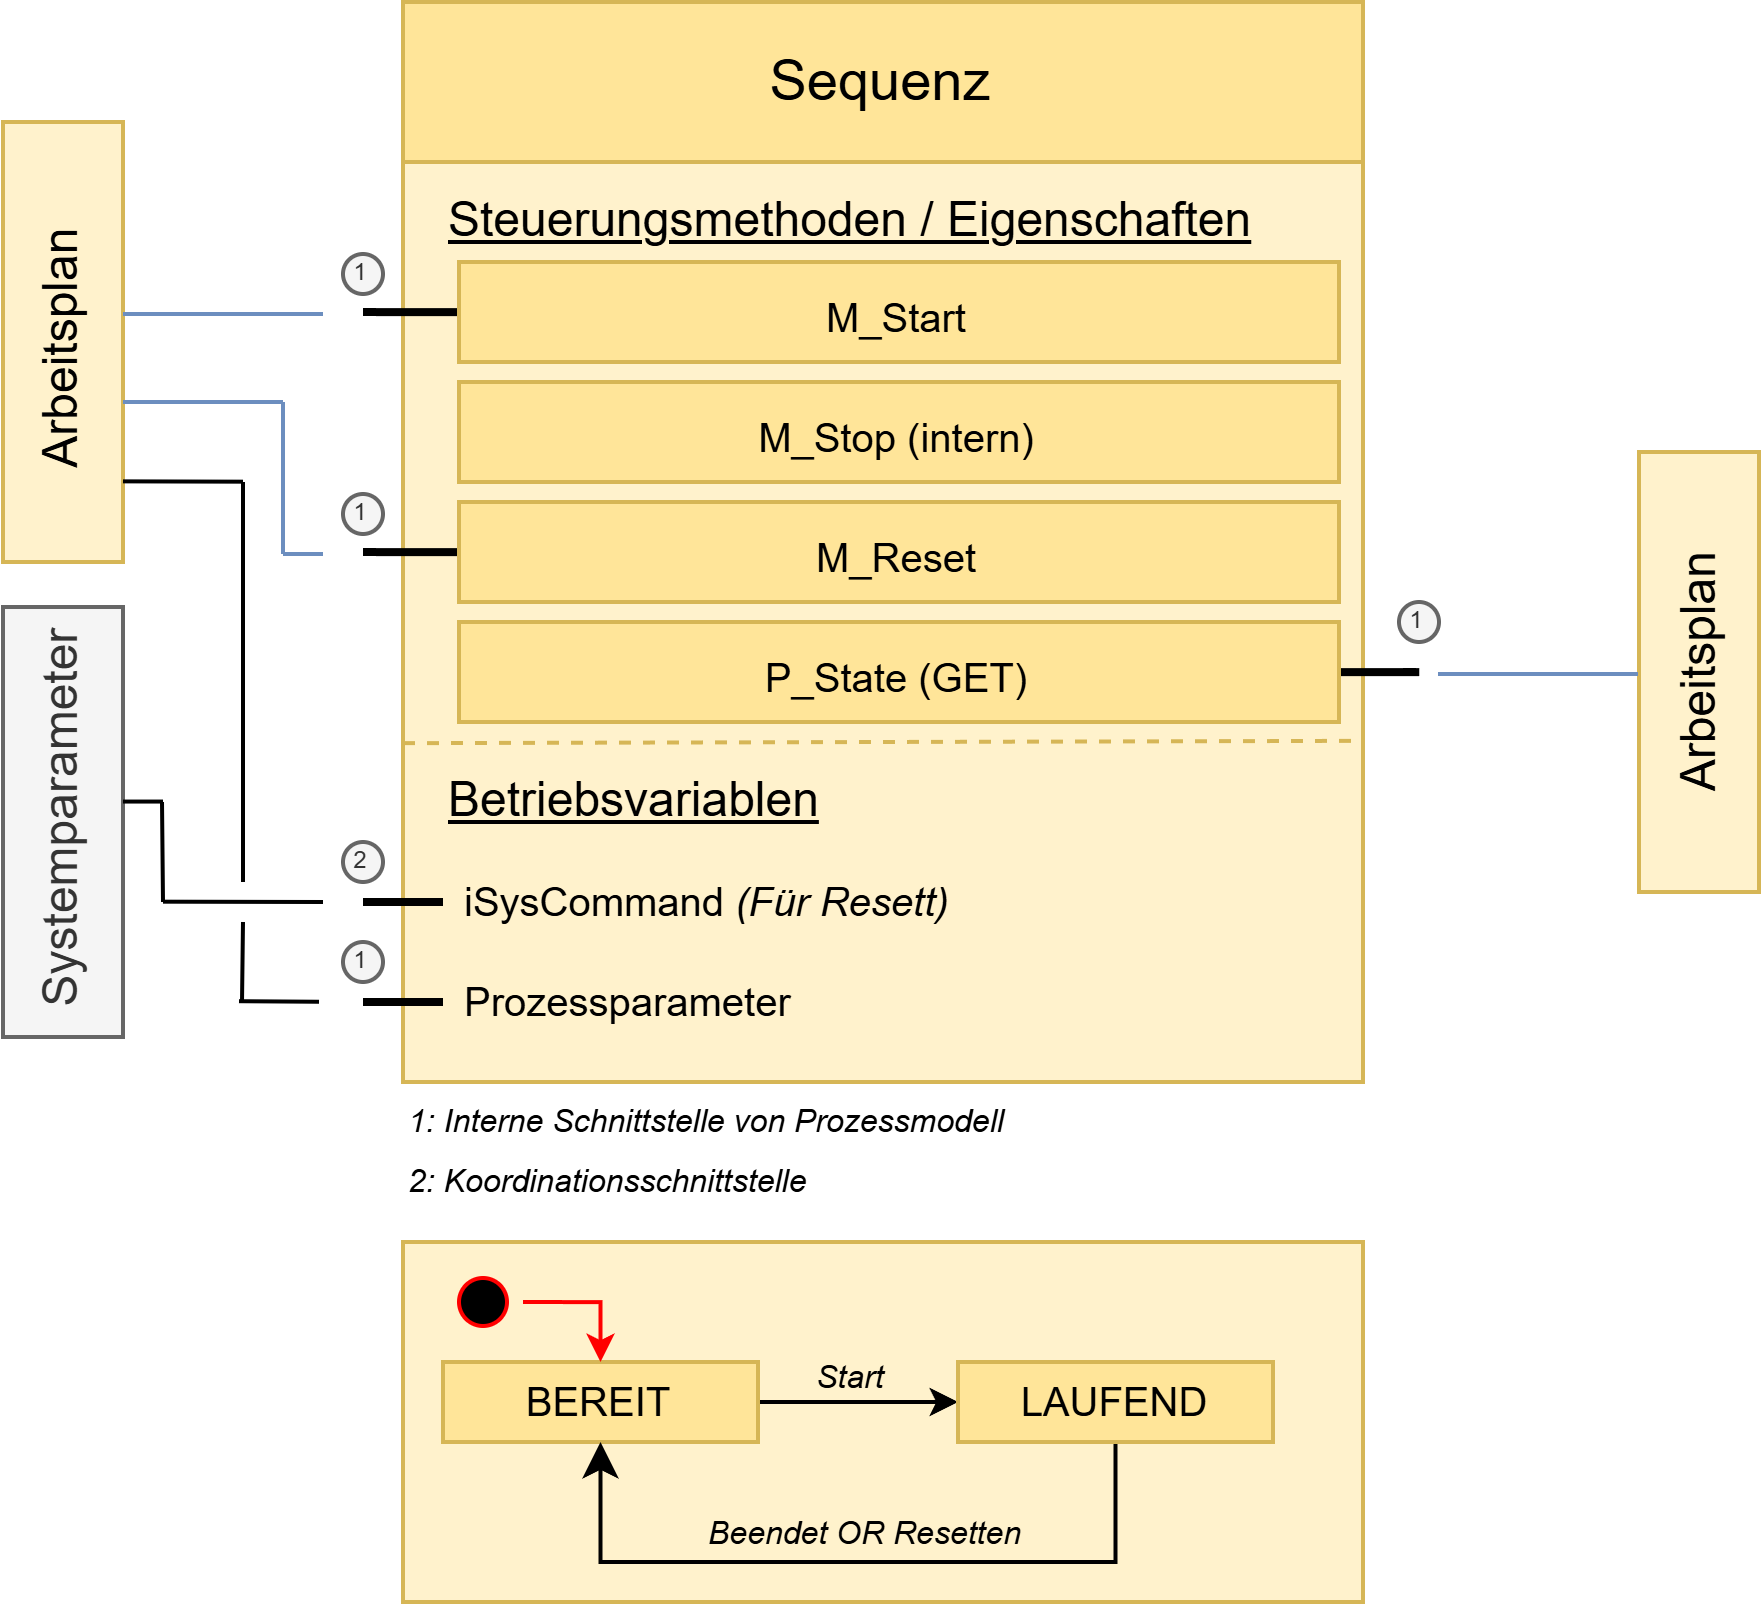
\includegraphics[width=.8\textwidth]{08_Prozessmodell/Sequenzstruktur}
			\captionsetup{justification=centering}
			\caption{Struktur einer Sequenz}
			\label{fig:Sequenzstruktur}
		\end{figure}
		
		Die Steuerungselemente umfassen die gleichen Methoden und Eigenschaften wie die Skills, die Umsetzung dieser unterscheidet sich jedoch. 
		
		\begin{table}[ht]
			\scriptsize
			\centering
			\colorlet{BFH-table}{BFH-MediumBlue!10}
			\colorlet{BFH-tablehead}{BFH-MediumBlue!50}
			\begin{bfhTabular}{llcl}
				Art: 		& Bezeichnung:	& Typ:			& Beschreibung:								
				\\\hline
				Methode		& \verb|M_Start|& \verb|BOOL|	& Methode zum Starten der Sequenz und des Schrittablaufs
				\\\hline
				Methode		& \verb|M_Stop|	& \verb|BOOL|	& Methode zum Beenden des Schrittablaufs (Intern)
				\\\hline
				Methode		& \verb|M_Reset|& \verb|BOOL|	& Methode zum Resetten der Sequenz und des Schrittablaufs
				\\\hline
				Eigenschaft	& \verb|P_State|& \verb|INT|	& Eigenschaft des aktuellen Zustandes
			\end{bfhTabular}
			\captionsetup{justification=centering}
			\caption{Steuerungselemente einer Sequenz}
			\label{tab:Sequenz_Steuerungselemente}
		\end{table}
		
		\newpage
		
	
	